\beginsong{Jalava}[
    wuw={Schmetterlinge}, 
    alb={Proletenpassion}, 
    jahr={1976}, 
    bo={346}, 
    pfii={44}, 
    pfiii={22}, 
    siru={243}, 
    tonspur={552}, 
    index={Von Sonn' und Kessel},
]

\beginverse
\endverse
\includegraphics[draft=false, width=1\textwidth]{Noten/Lied055.pdf}

\beginverse*
\endverse
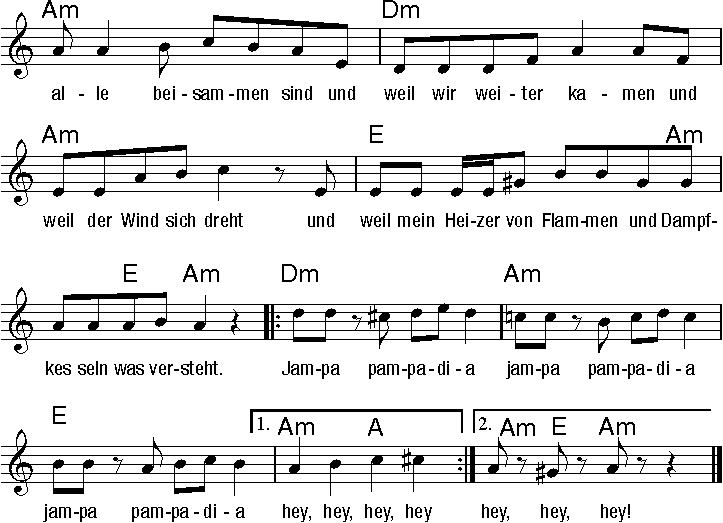
\includegraphics[draft=false, width=1\textwidth]{Noten/Lied055_1.pdf}	

\beginverse
Sie \[Am]dampften ein in Belostrow, wo Schocks von Offi\[E]zieren
die Züge auf dem Grenzbahnhof penibel kontrol\[Am]lieren.
Sie \[Dm]prüfen jegliches Gesicht bei \[Am]ihrer Inspizierung,
doch \[E]sehen sie am Kessel nicht den \[Am]Staatsfeind der Re\[E]gierung.
\[Am]Jalava weiß, worum es geht, und langsam dampft vor\[E]bei
am letzten Posten, der da steht, Lokomotive zwei-neun-\[Am]drei.
\endverse 

\beginchorus
\[Dm]Jalava, du Finne, was \[Am]lachst du gegen den Wind?
Ich \[E]lache, weil meine Sinne \[Am]alle beisammen sind
und \[Dm]weil wir weiterkamen und \[Am]weil der Wind sich dreht
und \[E]weil mein Heizer von Flammen und \[Am]Dampfkesseln \[E]was ver\[Am]steht.
\[Dm]Jam-pa pam-pa-di-a \[Am]jam-pa pam-pa-di-a \[E]jam-pa pam-pa-di-a \[Am]hey, hey, \[A]hey, hey
\[Dm]Jam-pa pam-pa-di-a \[Am]jam-pa pam-pa-di-a \[E]jam-pa pam-pa-di-a \[Am]hey, \[E]hey, \[Am]hey!
\endchorus

\beginverse
Da ^saust die Grenzstation vorbei, die Birken stehen ^nackt,
die Lokomotive zwei-neun-drei schnauft in erhöhtem ^Takt.
Und ^Jalava lacht in den Wind, in ^den Oktoberregen:
''^Heizer, wenn wir drüben sind, dann ^wird sich was be^wegen.''
Jetzt ^schneidet der Oktoberwind die letzten Äpfel ^an,
die an den kahlen Bäumen sind an der finnischen Eisen^bahn.
\endverse

\beginchorus
\[Dm]Jalava, du Finne, was \[Am]lachst du gegen den Wind?
Ich \[E]lache, weil meine Sinne \[Am]alle beisammen sind
und \[Dm]weil uns die Fahrt in den Bahnhof \[Am]hinter der Grenze führt
und \[E]Vladimir Iljitsch Uljanow, mein \[Am]Heizer, die \[E]Flammen \[Am]schürt.
\[Dm]Jam-pa pam-pa-di-a \[Am]jam-pa pam-pa-di-a \[E]jam-pa pam-pa-di-a \[Am]hey, hey, \[A]hey, hey
\[Dm]Jam-pa pam-pa-di-a \[Am]jam-pa pam-pa-di-a \[E]jam-pa pam-pa-di-a \[Am]hey, \[E]hey, \[Am]hey!
\endchorus

\endsong

\beginscripture{}
Das Jalava-Lied ist das bekannteste Lied der sogenannten Proletenpassion. Diese ist ein politsches Chorwerk aus dem Jahr 1976 mit dem Anspruch, die deutsche (Leidens-)Geschichte aus ihren Anfangstagen zu beschreiben. Das Jalava-Lied selbst beschreibt, wie Lenin vor der Oktoberrevolution, angeblich als Heizer verkleidet, auf einer finnischen Lokomotive über die Grenze nach Sankt Petersburg geschmuggelt wird.
\endscripture
